\section{Theorie}
\label{sec:Theorie}

\subsection{FACT}

The \textit{First G-APD Cherenkov Telescope} (FACT), depicted in figure \ref{fig:FACT}, is a ground based imaging cherenkov telescope. It was built in 2011 at the Observatorio 
del Roque los Muchachos, is operated remotely since 2012 and operates robotically since 2017.
The observed objects are the Crab-Nebula and mainly blazars. 
%
\begin{figure}[H]
    \centering
    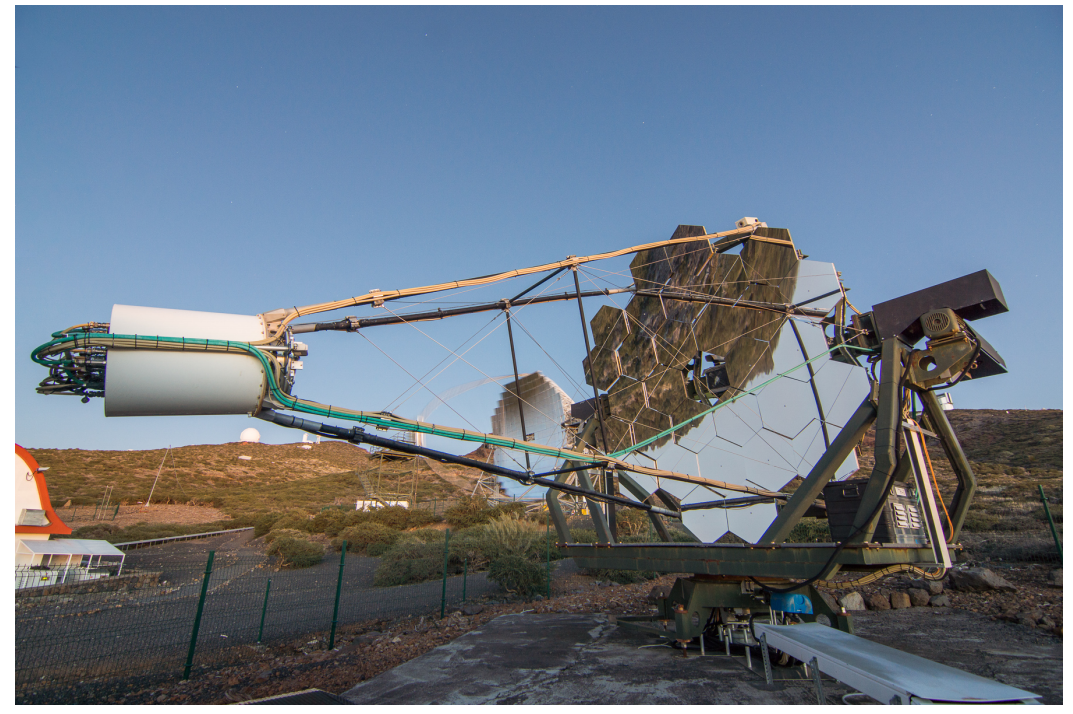
\includegraphics[width=0.7\textwidth]{graphics/FACT.png}
    \caption{The telescope FACT at the Observatorio del Roque los Muchachos on La Palma, Spain. \cite{sample}}
    \label{fig:FACT}
  \end{figure}
The telescope is operated in the wobble mode which enables it to observe sources of $\gamma$-radiation in the sky while also getting an estimate for the 
background radiation. In the mode it is aimed $0.6 °$ next to the observed source. The estimated region where the source is located is called the on-region 
while five geometrically equivalent points are selected, which are called off-regions, are selected to estimate the background as depicted in figure 
\ref{fig:OnOff}. 

\begin{figure}[H]
    \centering
    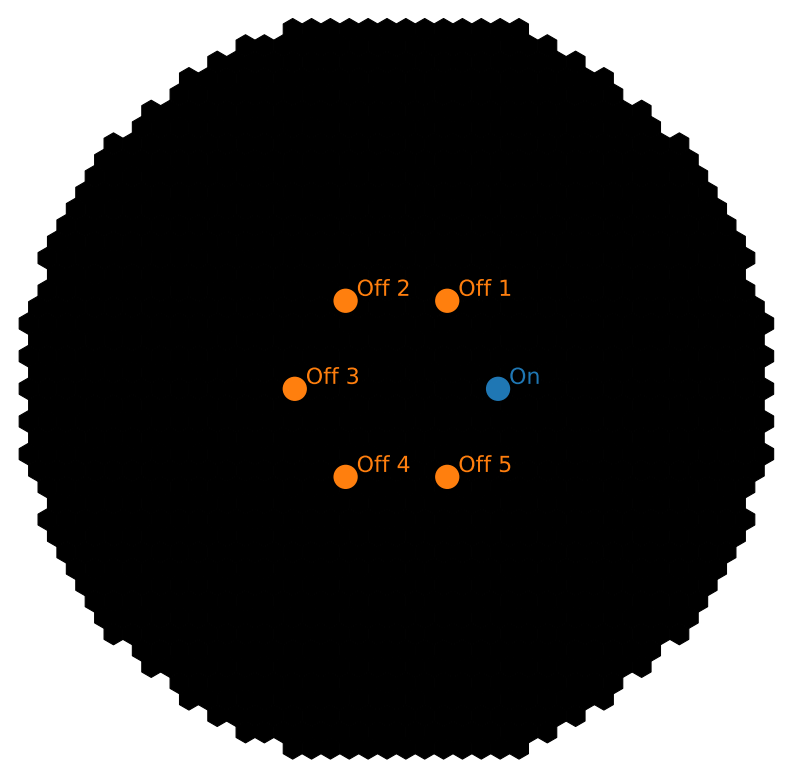
\includegraphics[width=0.5\textwidth]{graphics/OnOff.png}
    \caption{The field of view of FACT with the on- and the off-positions marked. \cite{sample}}
    \label{fig:OnOff}
\end{figure}

To calculate the significance of the measurement is calculated with the Likelihood-Ratio-Test 

\begin{equation}
    S = \sqrt{2} \cdot \sqrt{N_\text{on} \ln \biggl( \frac{1+ \alpha}{\alpha} \biggl( \frac{N_\text{on}}{N_\text{on} + N_\text{off}} \biggr) \biggr) 
    + N_\text{off} \ln \biggl( (1+\alpha) \frac{N_\text{off}}{N_\text{on} + N_\text{off} } \biggr) }
\end{equation}
where $N_\text{on}$ and $N_\text{off}$ are the numbers of reconstructed events in the on- and off-region respectively and $\alpha$ is the ratio of the number of 
on- and off-regions, therefore here $\alpha = \frac{1}{5}$.


\subsection{Deconvolution}

In experiment the physical quantities of interest are usually not measured directly but have to be extracted from the distribution of the signals 
produced by a detector $g(y)$ depending on an ensemble of observables $y$. 
This inverse problem can be written as the integral-equation 
\begin{equation}
    g(y) = \int A(y, \, x) f(x) \, dx + b(y)
\end{equation}
where $A(y, \, x)$ is the detector response function that describes how a physical quantites $x$ are converted into observables $y$ by the detector, $f(x)$ 
is the measured distribution of physical quantities to be extracted from the data and $b(y)$ is the background for the measurement. \\
One way to solve such a problem is to discretize the data to receiva an equation of the form 
\begin{equation}
    \vec{g} = \textbf{A} \cdot \vec {f} + \vec{b}
    \label{eq:disc_inv}
\end{equation}
where $\vec{g}$ and $\vec {b}$ are the $N$-dimensional vectors containing the histograms of the observable and the background, $\textbf{A}$ is the 
$M\times N$ migrationmatrix and $\vec{f}$ the $M$-dimensional vector containing the histogram of physical quantity of interest. \\
The goal here is to find an estimator $\hat{\vec{f}}(\textbf{A}, \, \vec{g}, \, \vec{b})$ with which the distribution of the pyhsical quantity of interest 
can be determined if $\textbf{A}$, $\vec{g}$ and $\vec{b}$ are known.

\subsubsection{Naive SVD-Deconvolution}

A method to solve the discretized inverse problem is to calculate the Moore-Penrose inverse of the migrationmatrix $\textbf{A}⁺$ and to rearrange 
equation \eqref{eq:disc_inv} to 
\begin{equation}
    \hat{\vec{f}} = \textbf{A}⁺ ( \vec{g} - \vec{b} ) .
\end{equation}

\subsubsection{Poisson-Likelihood-Deconvolution}
If one assumes the measured values $\vec{g}$ to be poisson distributed with 
\begin{equation}
    P(g_i) = \mathcal{P}(g_i , \, \lambda_i)
\end{equation}
being the probability for measuring $g_i$ where 
\begin{equation}
    \lambda_i = (\textbf{A} \cdot \vec {f} + \vec{b})_i 
\end{equation}
one can find an estimate for the values of $\vec{f}$ by maximizing the likelihood
\begin{equation}
    \mathcal{L} = \sum_{i=1}^M \mathcal{P}(g_i, \, \lambda_i) . 
\end{equation}
For numerical reasons it makes sense to consider minima of the negative log-likelihood 
\begin{equation}
    - \ln \mathcal{L} = \sum_{i=1}^M \biggl( \ln g_i! - g_i \cdot \ln \lambda_i + \lambda_i \biggr) . 
\end{equation}
If $\textbf{A}$, $\vec{g}$ and $\vec{b}$ are known this leads to the estimator 
\begin{equation}
    \hat{ \vec{f}} = \text{argmin} ( - \ln \mathcal{L} (f | \textbf{A}, \, \vec{g}, \, \vec{b})).
\end{equation}